\chapter{ATHENA} 

\label{Chapter2}

\section{Background}

ATHENA is a state-of-the-art, purpose-built system which is engineered by \textit{\groupname} at The University of Melbourne for the Australian Defence Science and Technology (DST) Group -- Training Analysis for Workforce Planning\footnote{\url{https://www.dst.defence.gov.au/research-facility/training-analysis-workforce-planning}} research centre. ATHENA is a strategic simulation and analysis system for manpower planning. The aim of the system is tackling workforce planning challenges of the Australian Defence Force (ADF) Training Continuum. 

To begin with, the project purpose is to develop the \textit{Dynamically Reconfigurable Agent-Based Discrete Event Simulator for Aircrew Training}. The project specification was originated in the ADF Helicopter Aircrew Training Continuum (HATC) system. The HATC\parencite{HATC} sytem is in a constant state of transience such that infrastructure consolidation -- e.g. phasing out of Aircraft, rules about criteria for passing individual training components, and changes in policies that govern training in individual schools and squadrons -- and, all these events occur rapidly. Changes like these are common in the system and, it inevitably causes perturbations in the flow of students through the training program. Therefore, it requires a framework designed to address the needs of ADF to perform \textbf{what-if scenario analysis}. To model such dynamic changes in the HATC complex system, while preserving a common simulation architecture, \parencite{HATC} identified the needs of reconfigurable simulation framework. Ever since, the HATC system evolved into ATHENA and, most recently in \parencite{8248116} discuss ATHENA as a more generic simulator for ADF manpower planning needs, such as not only for Pilot and Aircrew but also for Maritime Warfare Officer and Navy Submariner.
%to \textit{deal with manpower planning using a dynamic and interactive system that is agile and adaptive to robustly accommodate change -- without requiring a complete rewrite}.
These papers discuss the choice of Agent-Based Discrete Event Simulation (AB-DES) hybrid model and the details of the simulation modelling domain concept.

The remainder sections of this Chapter 2 focus more on the software engineering perspective and key excerpts from the ATHENA technical documentation v1.0 \parencite{athenaAllDoc}, an overview of the system, its architecture and major components, and highlight on Bag-of-Tasks (BoT) scaling potential for remote job execution.

\section{System Overview}

ATHENA provides facilities for simulation, visualisation and analysis. These three aspects come together to enable modelling, exploration and analysis of complex workforce and manpower resourcing scenarios.
\\
\\
%\subsection{Architecture}
\textbf{Architecture:} \quad ATHENA is a multi-user, multi-tier web application. Major components include the user interface, a backend web service, databases, a message broker, and simulation workers. Conceptually, the system follows a traditional 3-tier web application, as depicted in Figure~\ref{fig:conceptArch}. 

\begin{figure}[!htb]
\centering
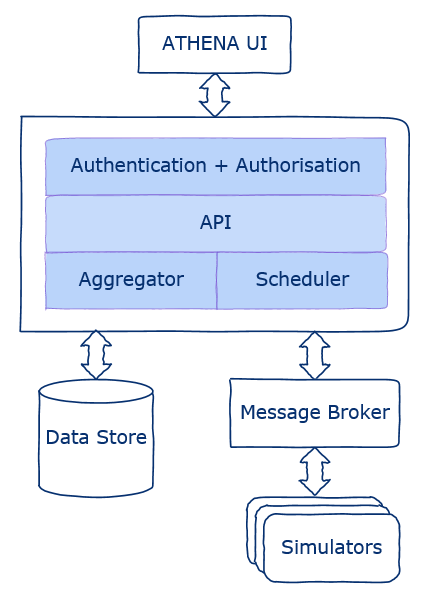
\includegraphics[width=0.4\textwidth]{Figures/ATHENA_conceptual_architecture}
\decoRule
\caption[ATHENA Conceptual Architecture]{Conceptual view of the multi-tier component architecture of the ATHENA system}
\label{fig:conceptArch}
\end{figure}

A user interface (UI), accessible via a web browser, provides access to the underlying modelling and simulation system. The user interface communicates with the backend system via REST\footnote{Representational State Transfer} API\footnote{Application Programming Interface} calls. These backend API calls are intercepted by an authentication and authorization layer, which perform user access control (ACL\footnote{Access Control List}) checks before despatching to various API endpoints. The backend system communicates with databases for the purpose of data persistence.

Apart from these traditional layers described above, the backend also communicates with a message broker for managing compute-intensive simulation tasks -- Bag-of-Tasks job execution using Enterprise Integration pattern --  Producer-Consumer Message-oriented architecture. These tasks are performed by a distributed set of workers, each hosting ATHENA's simulation engine.
\\
\\
%\subsection{Technology Stack}
\textbf{Technology Stack:} \quad Figure~\ref{fig:techStack} depicts ATHENA's technology stack. The backend service is a Spring framework-based modular application, written in Java. Primarily, the backend service provides logic related to the strategic aircrew training continuum, managing interfaces, business logic, data persistence, and distributed computation tasks. The data layer is composed of PostgreSQL RDBMS\footnote{Relational Database Management System}, which stores access control data, and document-oriented NoSQL MongoDB for storing all data related to the simulation model. Computation of simulations are performed by a network of lightweight workers, also written in Java, which communicate with the backend via JMS (Java Message Service). Apache ActiveMQ manages reliable delivery of messages containing simulation requests, results, and status updates. 

\begin{figure}
\centering
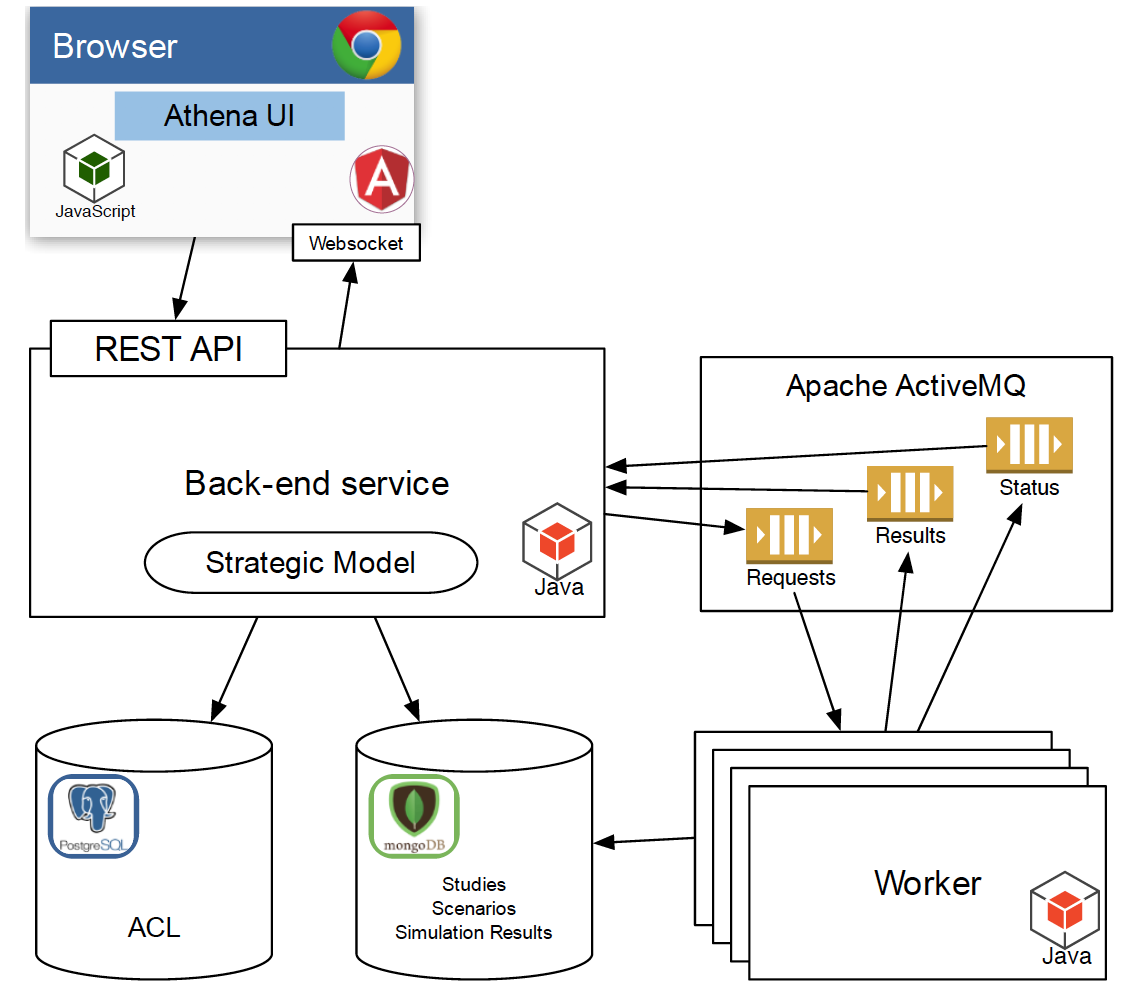
\includegraphics[width=0.5\textwidth]{Figures/ATHENA_tech_stack}
\decoRule
\caption[ATHENA Technology Stack]{ATHENA technology stack and their respective interactions}
\label{fig:techStack}
\end{figure}

The primary user interface is a AngularJS JavaScript Single-Page Application (SPA) loaded in an HTML5 compliant web browser. The UI communicates with the backend application server using both the HTTP REST API and WebSocket channels.

Figure~\ref{fig:scenarioScreen} shows a 10 year simulation result, the Scenario view which is the Sankey diagram\footnote{\url{https://en.wikipedia.org/wiki/Sankey_diagram}} (\textit{upper north}) -- visualisation of layered flow structure for the flow of the training continuum (\textit{left to right}). The Scenario Timeline (\textit{bottom south}) shows the statistical data of trainees or instructors over the whole simulation time span. The result also shows that the simulation have used \textbf{Monte Carlo} simulation and recruitment \textbf{optimisation algorithm} by labelling at the top left corner of the Sankey diagram.

\begin{figure}
\centering
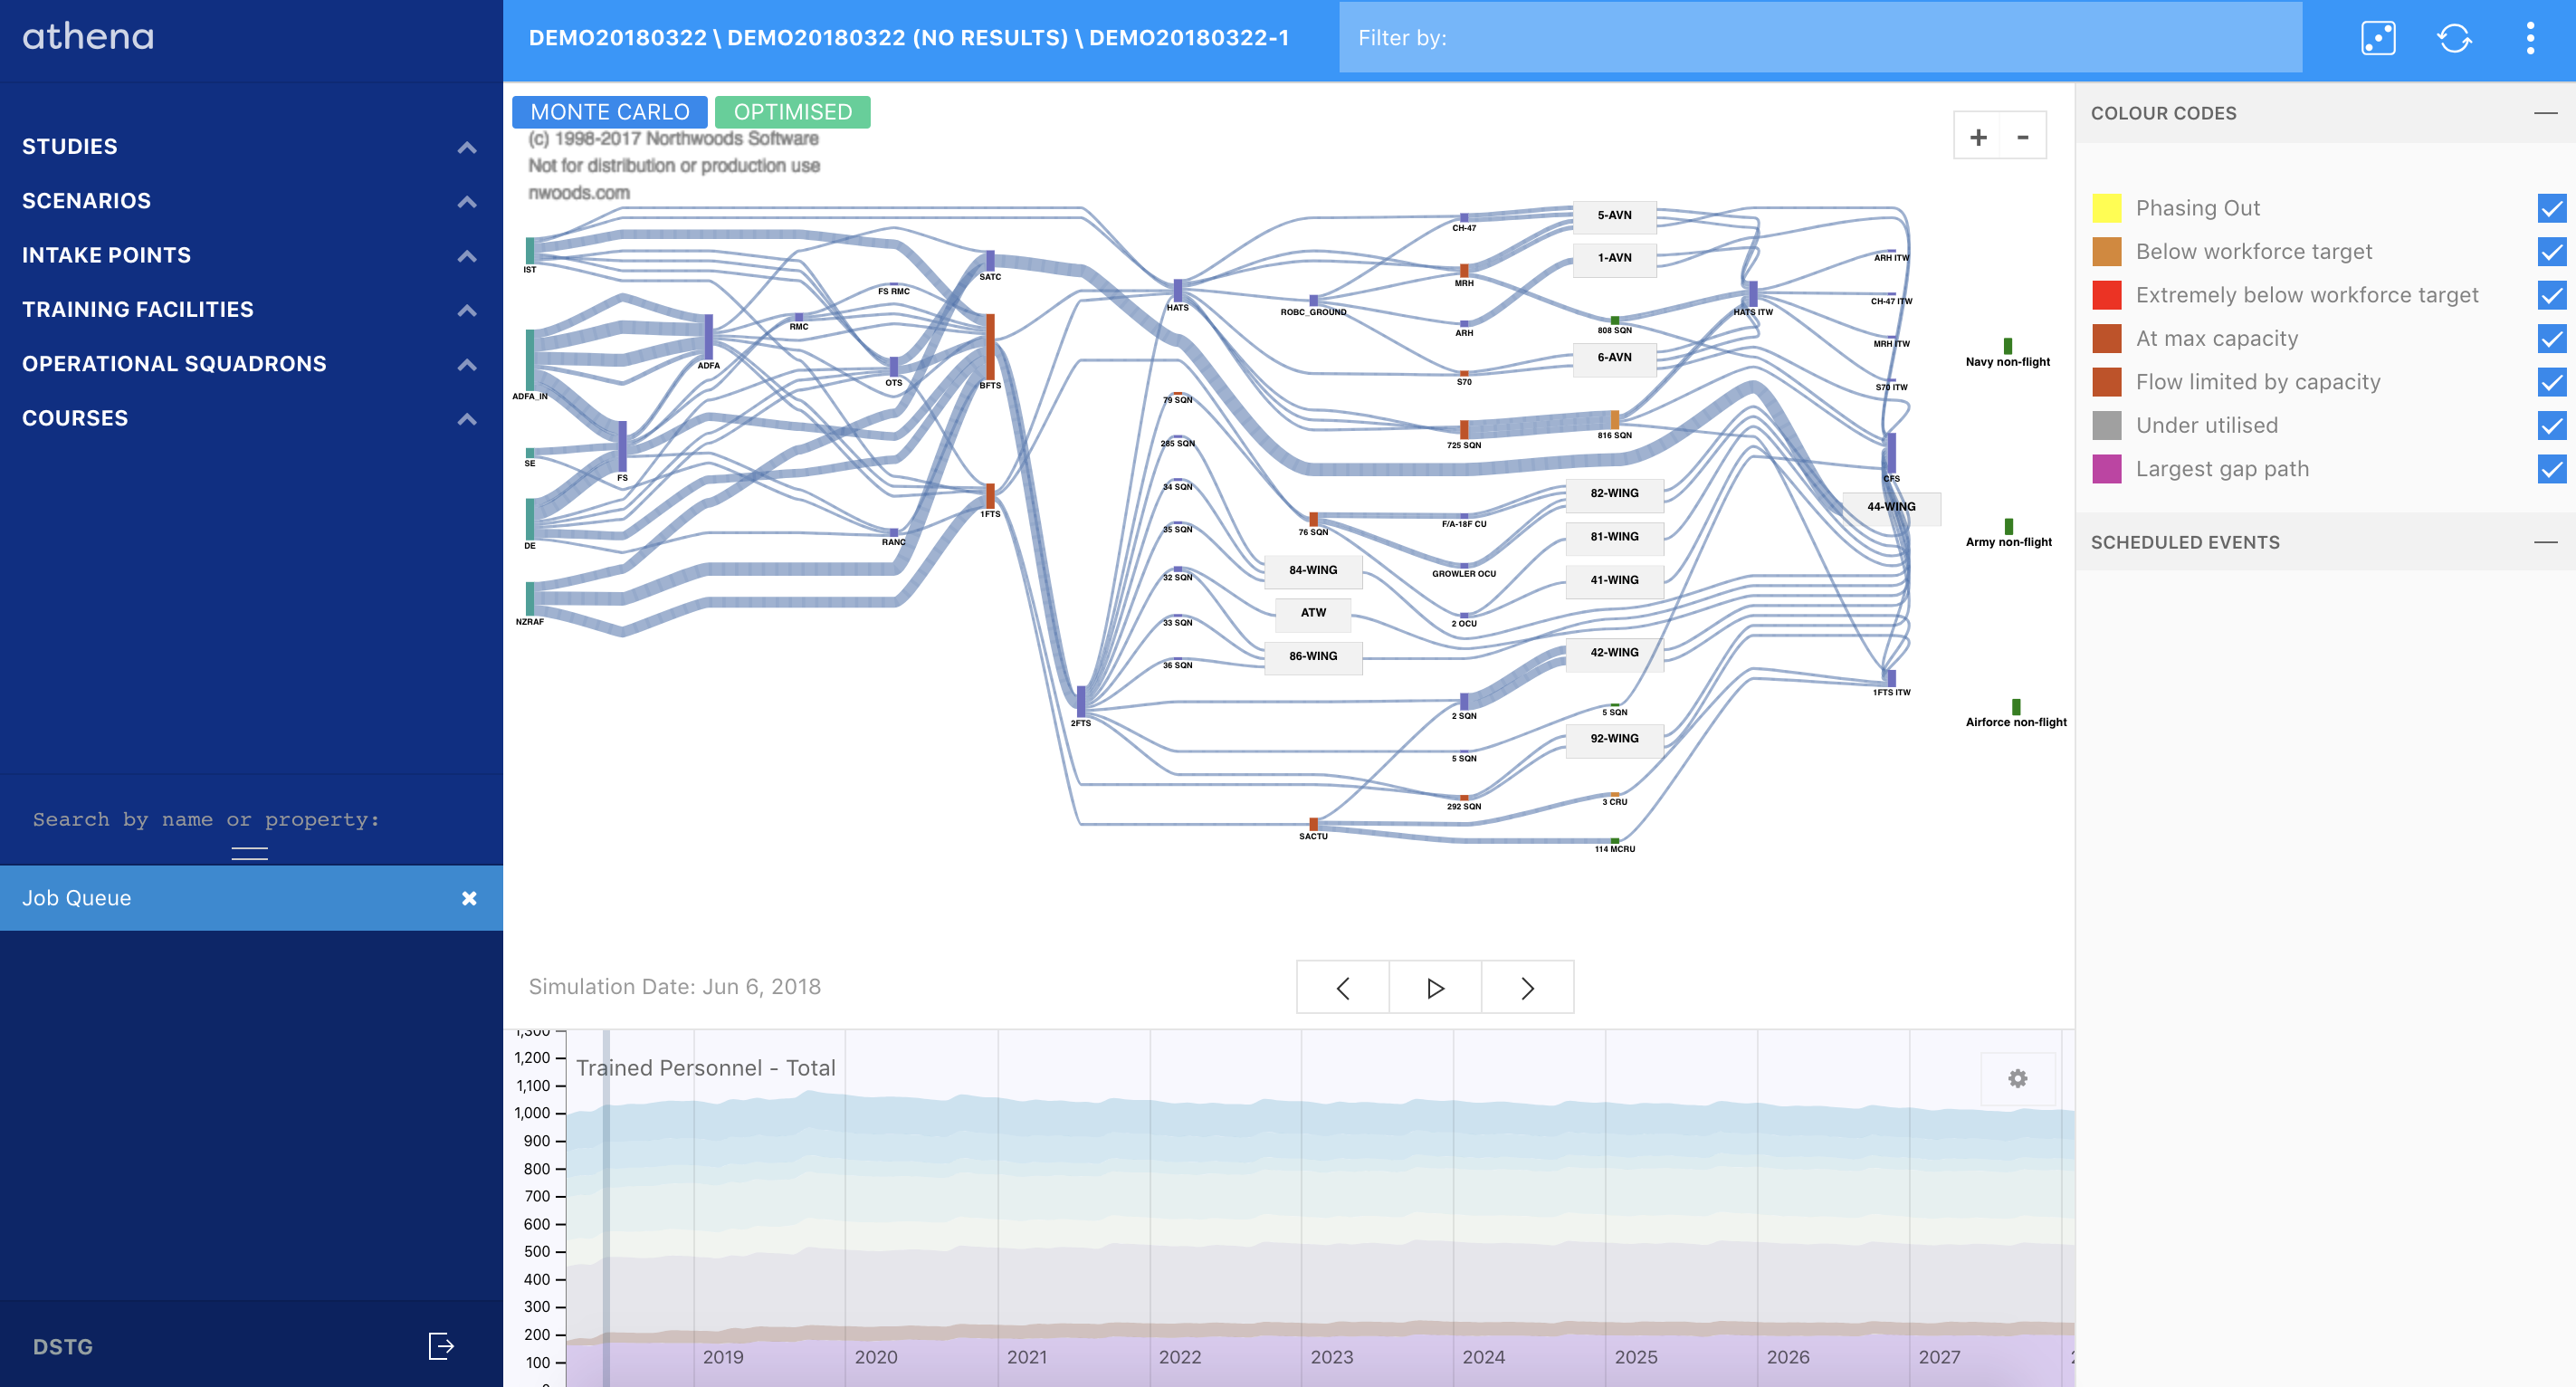
\includegraphics[width=0.8\textwidth]{Figures/ATHENA_scenario_screen}
\decoRule
\caption[ATHENA Scenario View]{ATHENA Scenario View}
\label{fig:scenarioScreen}
\end{figure}

\section{Remote Job Execution and Bag-of-Tasks Scaling Potential}

Simulation jobs can be computationally intensive, especially if one of the optimisation algorithms is activated. For this reason, a master-worker remote execution system has been designed aiming at offering high-performance and reliable simulations. Figure~\ref{fig:remoteJob} depicts this process.

\begin{figure}
\centering
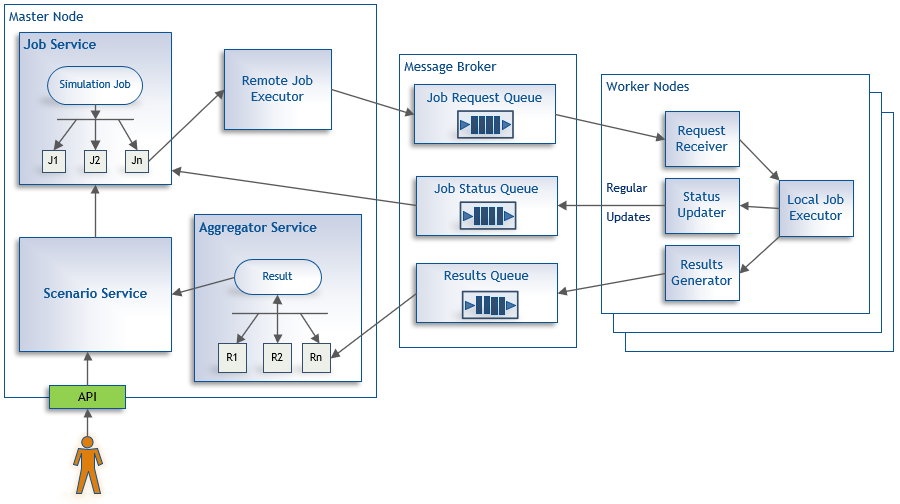
\includegraphics[width=0.8\textwidth]{Figures/ATHENA_remote_job_exec}
\decoRule
\caption[ATHENA Remote Job Execution]{ATHENA Process of remotely executing simulation jobs}
\label{fig:remoteJob}
\end{figure}

Monte-Carlo simulations, composed of many repetitions of the same process, are inherently a good fit for this system due to their embarrassingly parallel nature. 
In the master node, the job execution system is composed of a modular set of services. Once a scenario is submitted for simulation, the \textbf{Scenario Service} deals with assembling a simulation model with the correct inputs and creates one sub-scenarios for each Monte-Carlo repetition. Effectively, the simulation is parallelised into \textit{N} independent jobs, created by the \textbf{Job Service}, which is responsible for managing the job state, i.e. creating, updating and cancelling job executions. The \textbf{Remote Job Executor} interfaces with the \textbf{Message Broker} via the JMS protocol. At this point, the \textbf{Job Request Queue} will contain multiple job definitions, ready to be consumed by workers. 
There can be many worker nodes, which consume messages from the \textbf{Job Request Queue}, interpret the job definition, read job inputs, and perform local execution of the simulation model. As jobs are dequeued, start and finish execution, the worker sends status updates via the \textbf{Job Status Queue}, which are in turn consumed by the master in order to provided progress updates to the end-user. Each individual simulation repetition produces one result instance, or intermediate result. These are send via the \textbf{Results Queue} and consumed by an \textbf{Aggregator Service} that performs statistical aggregation, thus producing the mean and confidence intervals of all model statistics over all simulation runs. The execution is reliable in the sense that the failure of a worker does not cause the entire simulation to fail, as failed jobs are simply retried by another available worker. 
\\
\\
\\
For further details, readers are recommended to read the complete documentations of the ATHENA system in \parencite{athenaAllDoc}.
